\documentclass{recipe}

\begin{document}
\begin{recipe}{Coq Au Vin}
  \servings{3}

  \begin{ingredients}
    \ingredient{2}{slices}{bacon}
    \ingredient{3}{}{chicken thighs}
    \ingredient{2}{tbsp}{butter}
    \ingredient{1}{}{spanish onion}
    \ingredient{}{}{salt}
    \ingredient{1}{tbsp}{flour}
    \ingredient{}{}{herbs de provene}
    \ingredient{5}{oz}{red wine}
    \ingredient{8}{oz}{fettuchini}
  \end{ingredients}

  \begin{images}
    \begin{image}
      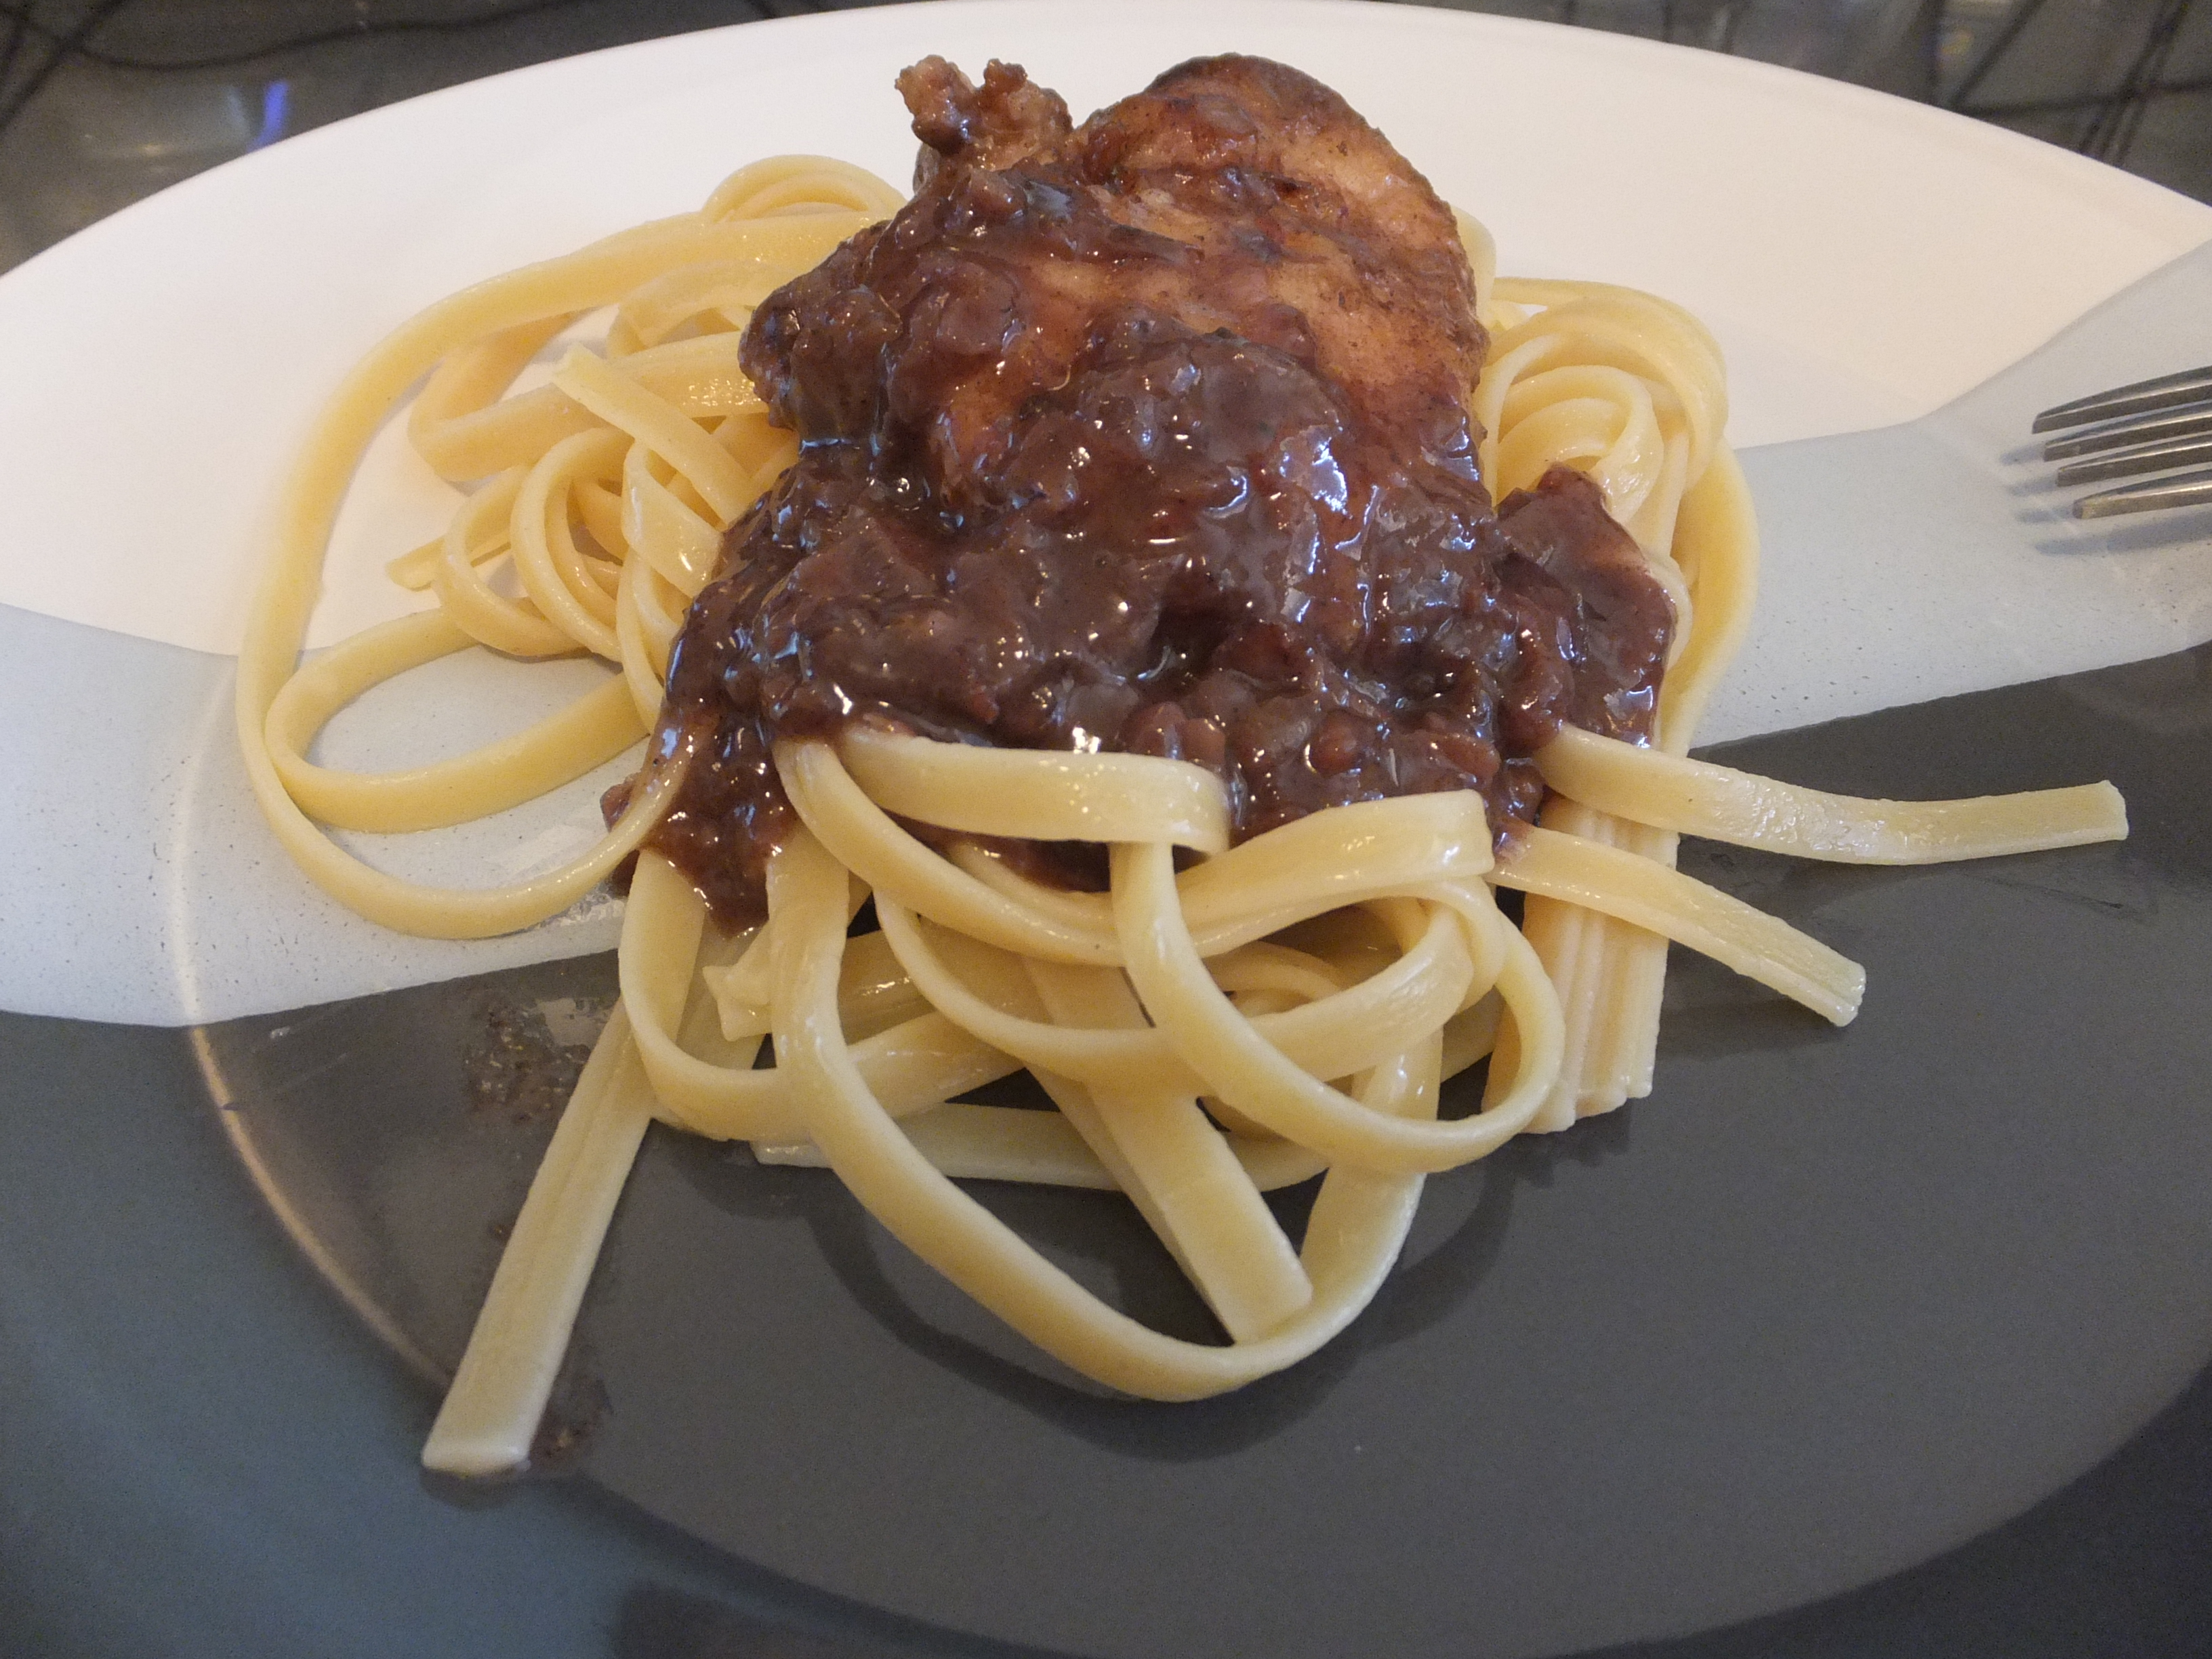
\includegraphics[width=\linewidth,trim=400px 400px 200px 500px, clip=true]{coq_a_vin-01.jpeg}
    \end{image}
  \end{images}

  \begin{steps}
  \item Dry the chicken thighs and dredge them in flour.
  \item Slice the bacon fairly small and cook it in the pan until all
    the fat is released.
  \item Remove the bacon from the pan, leaving the fat.
  \item Brown the chicken thighs in the bacon fat (and maybe some
    additional butter, but you might also have to remove some bacon
    fat) on both sides.
  \item Mince the onion
  \item Remove the chicken thighs from the pan, leaving any residual
    fat.
  \item Thoroughly cook the onion with some salt and butter
  \item Add some flour and a bit of butter to the onions, and cook the
    flour out.
  \item Deglaze the pan with the wine, slowly mixing it into the
    flour-onion mixture.
  \item Braise the chicken in the wine for about half an hour.
  \item Serve with pasta.
  \end{steps}

  \begin{notes}
  \item It's best to use the bone-in, skin-on chicken thighs, but the
    photo is from the plain ones (they're just tasteless).
  \item The cooking times are listed for the boneless, skinless thighs
    -- the good ones could stand a bit longer cooking time (maybe an
    hour).
  \item I put in way too much flour, but I put in more than that
    tablespoon so this is sort of a guess.
  \end{notes}
\end{recipe}
\end{document}
